
% v2-acmsmall-sample.tex, dated March 6 2012
% This is a sample file for ACM small trim journals
%
% Compilation using 'acmsmall.cls' - version 1.3 (March 2012), Aptara Inc.
% (c) 2010 Association for Computing Machinery (ACM)
%
% Questions/Suggestions/Feedback should be addressed to => "acmtexsupport@aptaracorp.com".
% Users can also go through the FAQs available on the journal's submission webpage.
%
% Steps to compile: latex, bibtex, latex latex
%
% For tracking purposes => this is v1.3 - March 2012
\documentclass[prodmode,acmtecs]{acmsmall} % Aptara syntax
\usepackage[spanish,polish]{babel}
\usepackage[T1]{fontenc}
\usepackage{fancyvrb}
\usepackage{graphicx,hyperref}
\newcommand\cutout[1]{}


\usepackage[table]{xcolor}
\usepackage[utf8]{inputenc}
\usepackage[parfill]{parskip}
\usepackage{tabulary}
\PassOptionsToPackage{hyphens}{url}
\usepackage{hyperref}    
\usepackage[capitalize]{cleveref}


% Metadata Information
% !!! TODO: SET THESE VALUES !!!
\acmVolume{0}
\acmNumber{0}
\acmArticle{CFP}
\acmYear{0}
\acmMonth{0}

\newcounter{colstart}
\setcounter{page}{4}

\RecustomVerbatimCommand{\VerbatimInput}{VerbatimInput}%
{
%fontsize=\footnotesize,
fontfamily=\rmdefault
}


\newcommand{\UnderscoreCommands}{%\do\verbatiminput%
\do\citeNP \do\citeA \do\citeANP \do\citeN \do\shortcite%
\do\shortciteNP \do\shortciteA \do\shortciteANP \do\shortciteN%
\do\citeyear \do\citeyearNP%
}

\usepackage[strings]{underscore}



% Document starts
\begin{document}


\setcounter{colstart}{\thepage}

\acmArticle{CFP}
\title{{\huge\sc SIGLOG Monthly 237}

 May 2023}
\author{DAVID PURSER\affil{University of Liverpool, UK}
\vspace*{-2.6cm}\begin{flushright}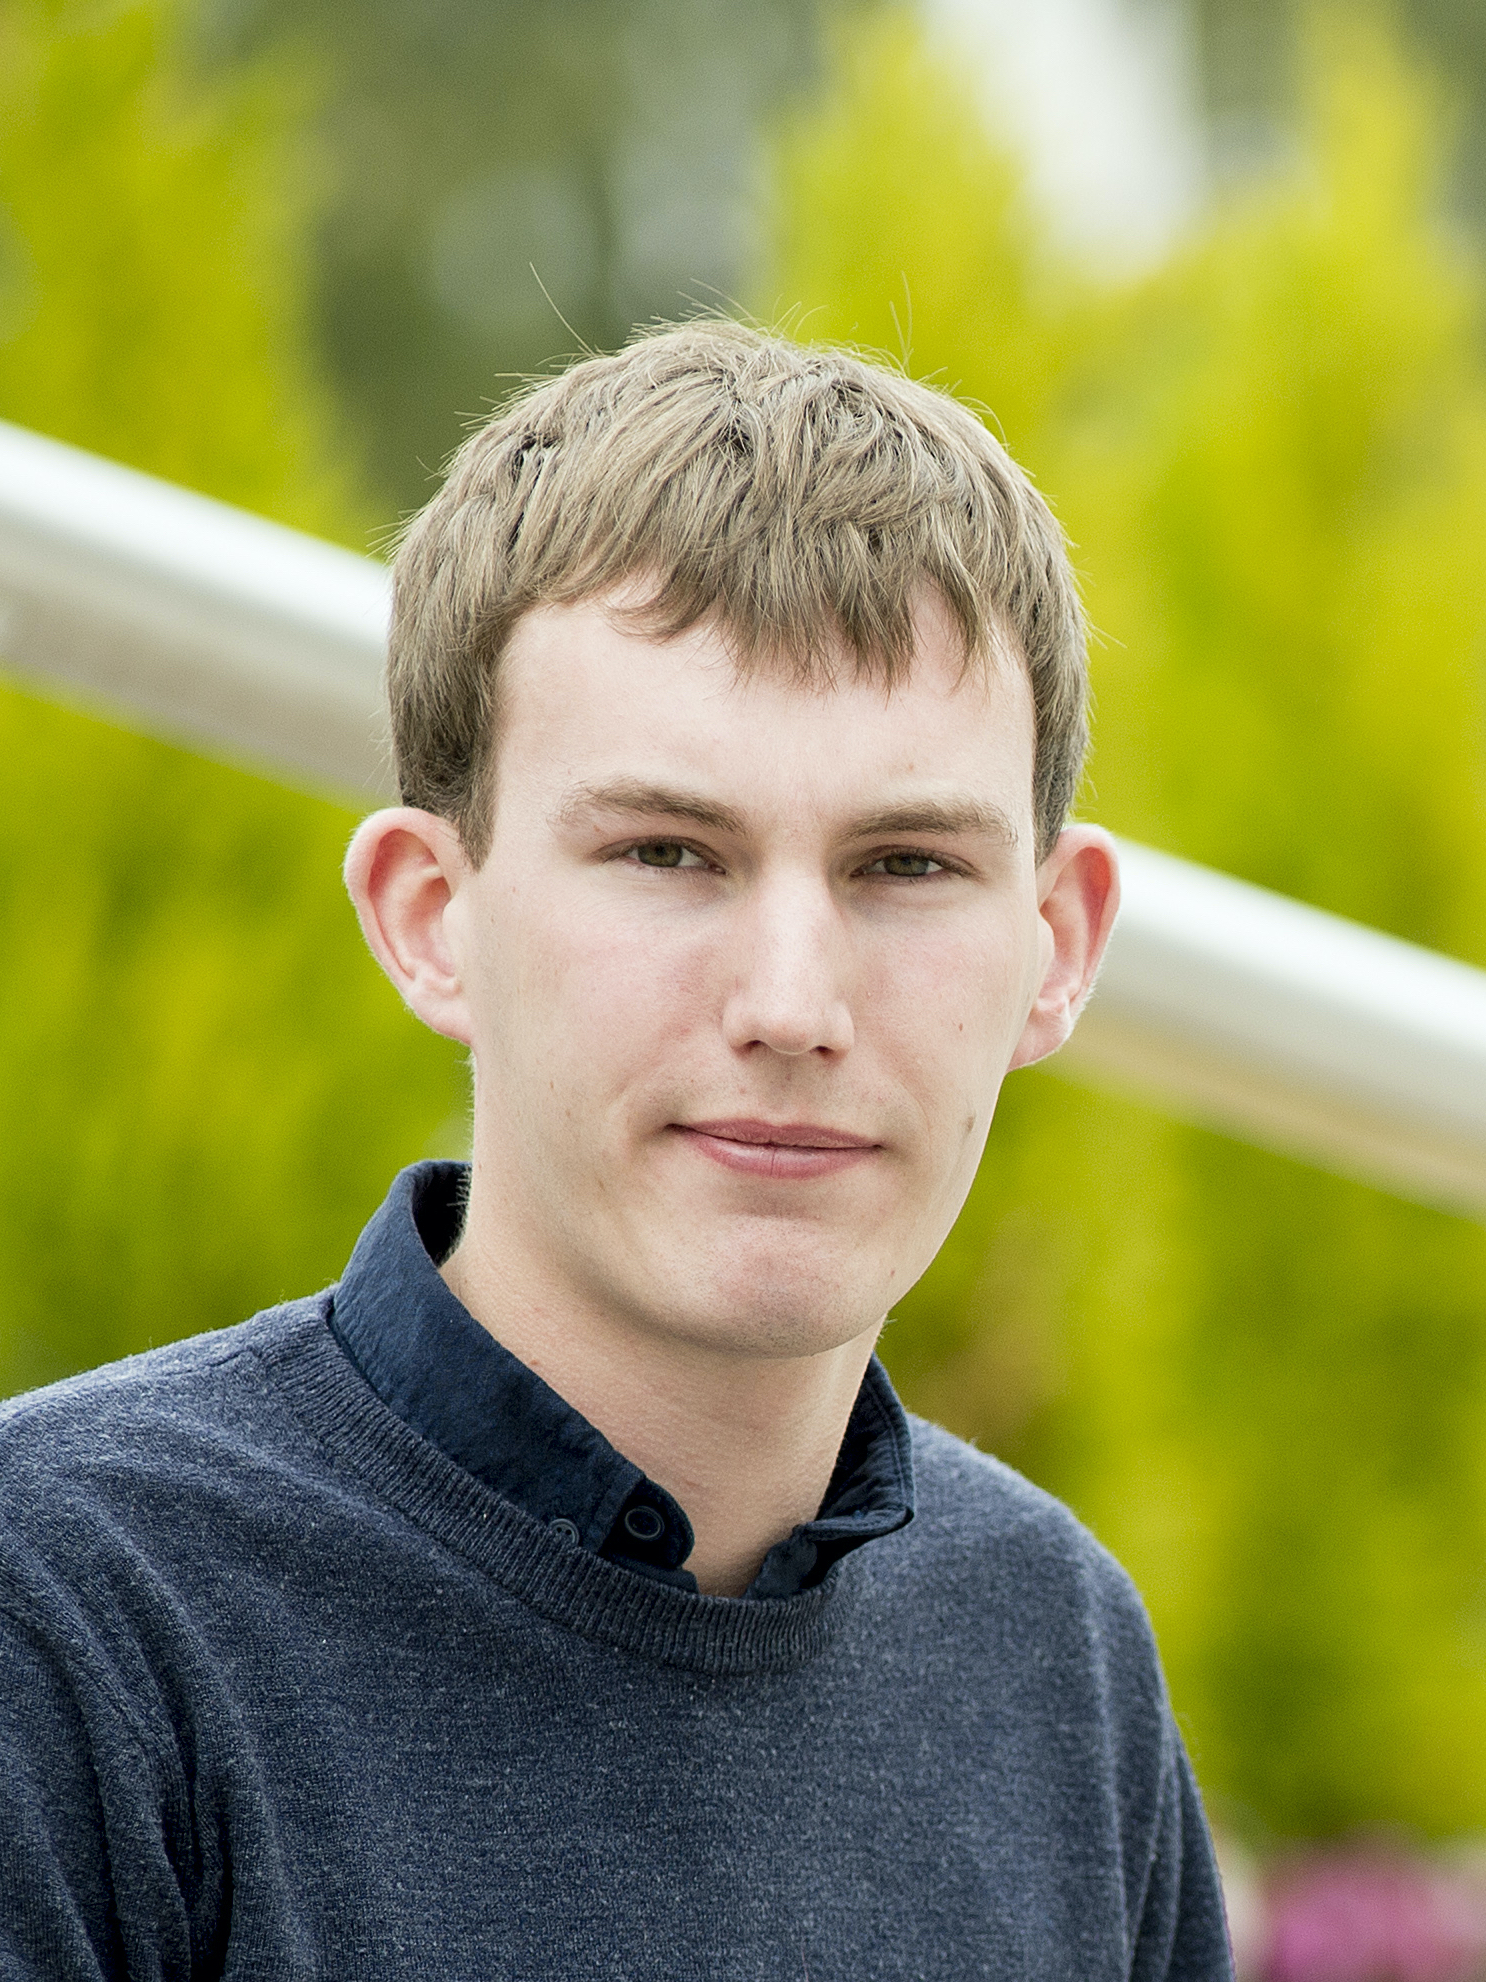
\includegraphics[width=30mm]{dp}\end{flushright}
}

\begin{abstract}
May 2023 edition of SIGLOG Monthly, featuring deadlines, calls and community announcements.
\end{abstract}


\maketitlee

\href{https://lics.siglog.org/newsletters/}{Past Issues}
 - 
\href{https://lics.siglog.org/newsletters/inst.html}{How to submit an announcement}
\section{Table of Content}\begin{itemize}\item DEADLINES (\cref{deadlines}) 
 
\item SIGLOG MATTERS 
 
\begin{itemize}\item LICS 2023 (\cref{LICS2023})
\end{itemize} 
\item CALLS 
 
\begin{itemize}\item WPTE 2023 (CALL FOR PAPERS / DEADLINE EXTENSION) (\cref{WPTE2023})
\item ZJULogAI 2023 (CALL FOR PAPERS) (\cref{ZJULogAI2023})
\item The Proof Society Workshop on Proof Theory and its Applications (CALL FOR PAPERS) (\cref{TheProofSocietyWorkshoponProofTheoryanditsApplications})
\item ASPOCP 2023 (CALL FOR PAPERS) (\cref{ASPOCP2023})
\item MOSAIC 2023 (CALL FOR PAPERS) (\cref{MOSAIC2023})
\item SEFM'23 (CALL FOR PAPERS) (\cref{SEFM23})
\end{itemize} 
\item JOB ANNOUNCEMENTS 
 
\begin{itemize}\item Proof Assistant Postdoc at University of Sheffield (\cref{ProofAssistantPostdocatUniversityofSheffield})
\item Associate Professor or Professor at Università degli Studi di Verona (\cref{AssociateProfessororProfessoratUniversitdegliStudidiVerona})
\end{itemize} 
\end{itemize}\section{Deadlines}\label{deadlines}\rowcolors{1}{white}{gray!25}\begin{tabulary}{\linewidth}{LL}LICS 2023 Workshop on Combinatorial Games in Finite Model Theory:  & May 01, 2023 (Abstract Submission) \\
HOR 2023:  & May 02, 2023 (Submission deadline) \\
ACT 2023:  & May 03, 2023 (Submission Deadline) \\
FORMATS 2023:  & May 04, 2023 (Abstract, extended), May 08, 2023 (Paper, extended) \\
WPTE 2023:  & May 05, 2023 (Paper, extended) \\
CLAR 2023:  & May 06, 2023 (Submission deadline, extended) \\
GCM 2023:  & May 07, 2023 (Abstract), May 14, 2023 (Paper) \\
TIME 2023:  & May 12, 2023 (Abstract, extended), May 19, 2023 (Paper, extended) \\
RSSRail 2023:  & May 12, 2023 (Papers and Abstract for tutorials, extended) \\
LORI 2023:  & May 15, 2023 (Paper deadline) \\
The Proof Society Workshop on Proof Theory and its Applications:  & May 15, 2023 (Submission deadline) \\
ASPOCP 2023:  & May 15, 2023 (Abstract), May 22, 2023 (Paper) \\
MOSAIC 2023:  & May 15, 2023 (Submission deadline) \\
EUMAS 2023:  & May 20, 2023 (Papers) \\
Proof Assistant Postdoc at University of Sheffield:  & May 23, 2023 (Closing date for applications) \\
iFM 2023:  & May 25, 2023 (Abstract) \\
FSCD 2025:  & May 27, 2023 (Deadline for location proposals) \\
Associate Professor or Professor at Università degli Studi di Verona:  & May 30, 2023 (Recommended deadline) \\
ESSLLI:  & May 31, 2023 (Early-registration deadline) \\
Two open positions of logic at Zhejiang University in 2023:  & May 31, 2023 (Application deadline) \\
SEFM'23:  & Jun 02, 2023 (Abstract), Jun 09, 2023 (Paper) \\
GandALF 23:  & Jun 23, 2023 (Abstract), Jun 30, 2023 (Paper) \\
ACKERMANN AWARD 2023:  & Jul 01, 2023 (Deadline for) \\
ICDT 2024:  & Sep 13, 2023 (Cycle 2 Abstract), Sep 20, 2023 (Cycle 2 Full) \\
\end{tabulary}
\section{LICS 2023: Thirty-Eighth Annual ACM/IEEE Symposium on LOGIC IN COMPUTER SCIENCE}\label{LICS2023}  26 June – 29 June 2023 preceded by workshops 24-25 June 2023\\ 
  \href{https://lics.siglog.org/lics23/}{https://lics.siglog.org/lics23/}\\ 
CALL FOR PARTICIPATION 

\begin{itemize}\item  Links to registration and local information: 
 
  \href{https://lics.siglog.org/lics23/registration.php}{https://lics.siglog.org/lics23/registration.php} 
 
  \href{https://lics.siglog.org/lics23/logistics.php}{https://lics.siglog.org/lics23/logistics.php} 
 
  Do book accommodation sooner rather than later. Boston can be expensive and there is another big event on 25 June.  
 
\item  List of accepted papers: \href{https://lics.siglog.org/lics23/accepted.php}{https://lics.siglog.org/lics23/accepted.php} 
 
\item  Invited talks and tutorials from Adnan Darwiche, Azadeh Farzan, Dale Miller, Toniann Pitassi, Dan Suciu 
 
\item  Workshops: 
 
\begin{itemize}\item  Combinatorial games in finite model theory
\item  The decision problem in first order logic (DPFO 2023)
\item  International Workshop on Quantitative Logical Methods (Qualog) 
\item  Structure meets power
\item  Logic mentoring workshop (LMW)
\end{itemize} 
\end{itemize}\section{WPTE 2023: 10th International Workshop on Rewriting Techniques for Program Transformations and Evaluation}\label{WPTE2023}  July 1, 2023, Rome, Italy\\ 
  \href{https://wpte2023.github.io/}{https://wpte2023.github.io/}\\ 
  \href{https://easychair.org/conferences/?conf=wpte2023}{https://easychair.org/conferences/?conf=wpte2023}\\ 
CALL FOR PAPERS / DEADLINE EXTENSION 

\begin{itemize}\item  The aim of WPTE is to bring together the researchers working on program transformations, evaluation, and operationally based programming language semantics, using rewriting methods, in order to share the techniques and recent developments and to exchange ideas to encourage further activation of research in this area. 
 
\item  Topics include: correctness of program transformations, optimizations and translations; program transformations for proving termination, confluence, and other properties; correctness of evaluation strategies; operational semantics of programs, operationally-based program equivalences such as contextual equivalences and bisimulations; cost-models for arguing about the optimizing power of transformations and the costs of evaluation; program transformations for verification and theorem proving purposes; translation, simulation, equivalence of programs with different formalisms, and evaluation strategies; program transformations for applying rewriting techniques to programs in specific programming languages; program transformations for program inversions and program synthesis; program transformation and evaluation for Haskell and rewriting. 
 
\item  Important dates: 
 
\rowcolors{1}{white}{gray!25}\begin{tabulary}{\linewidth}{LL}Paper submission, extended:  & May 05, 2023 \\
Notifications:  & Jun 05, 2023 \\
Final version for informal proceedings:  & Jun 18, 2023 \\
Workshop:  & Jul 01, 2023 \\
Submission to post-proceedings (journal):  & autumn 2023 (tbc) \\
\end{tabulary}
 
\end{itemize}\section{ZJULogAI 2023: Zhejiang University Logic and AI Summit}\label{ZJULogAI2023}  8th - 12th September 2023 Hangzhou (China)\\ 
CALL FOR PAPERS 

\begin{itemize}\item  Zhejiang University Logic and AI Summit (ZJULogAI 2023) brings together the 5th International Conference on Logic and Argumentation (CLAR 2023), the 3rd International Workshop on Logics for New-Generation Artificial Intelligence (LNGAI 2023), International Workshop on Logic, AI and Law (LAIL 2023), the workshop on Epistemology \& AI, and the workshop on AI \& Arts. It will take place at Zhejiang University on September 8th – 12th, 2023. See the venue information for details. 
 
  With its special focus theme on “methods and tools for explainable and ethical AI”, a core objective of ZJULogAI is to present the latest developments and progress made on the crucial question of how to make AI more interpretable, explainable, legal and ethical. 
 
  There are multiple events: 
 
\item   Epistemology \& AI 
 
\begin{itemize}\item  Event Dates: 8th - 9th September 2023  
\item  Submission Deadline: 15th May 2023
\item  Web page: \href{https://www.zlaire.net/zjulogai2023/epistemology\&ai2023}{https://www.zlaire.net/zjulogai2023/epistemology\&ai2023} 
\end{itemize} 
\item   LNGAI 
 
\begin{itemize}\item  Event Dates: 8th - 9th September 2023
\item  Submission Deadline: 1st May 2023
\item  Web page: \href{https://www.zlaire.net/zjulogai2023/lngai2023/}{https://www.zlaire.net/zjulogai2023/lngai2023/}
\end{itemize} 
\item   CLAR:  
 
\begin{itemize}\item  Event Dates: 10th - 12th September 2023 
\item  Submission Deadline: 6th May 2023 (extended)
\item  Web page: \href{https://www.zlaire.net/zjulogai2023/clar2023/}{https://www.zlaire.net/zjulogai2023/clar2023/} 
\end{itemize} 
\item   LAIL 
 
\begin{itemize}\item  Event Dates: 11th - 12th September 2023
\item  Submission Deadline: 8th May 2023
\item  Web page: \href{https://www.zlaire.net/zjulogai2023/lail2023}{https://www.zlaire.net/zjulogai2023/lail2023}
\end{itemize} 
\item   AI \& Arts 
 
\begin{itemize}\item  11th September 2023 (tentative)
\end{itemize} 
\end{itemize}\section{The Proof Society Workshop on Proof Theory and its Applications}\label{TheProofSocietyWorkshoponProofTheoryanditsApplications}  13-14 July, 2023\\ 
  Downtown Barcelona, Catalonia, Spain\\ 
  \href{https://www.ub.edu/prooftheory/event/tps2023/}{https://www.ub.edu/prooftheory/event/tps2023/}\\ 
CALL FOR PAPERS 

\begin{itemize}\item  The workshop is aimed at PhDs and other professionals alike. We call for contributed papers to be presented during the workshop either in a short talk of about 20 minutes or through a poster presentation. 
 
\item  IMPORTANT DATES 
 
\rowcolors{1}{white}{gray!25}\begin{tabulary}{\linewidth}{LL}Submission deadline:  & May 15, 2023 \\
Author notification:  & May 29, 2023 \\
\end{tabulary}
 
\item  SUBMISSION 
 
  Submissions consist of an extended abstract of at most four pages total (including references, acknowledgements, and any possible appendices). Accepted abstracts will be distributed during the event and may be posted, but will not be formally published, so we welcome work published elsewhere. Shortly we shall send out instructions on the format and method of submission. 
 
\item  AIMS AND SCOPE 
 
  Topics presented include. but are not limited to 
 
\begin{itemize}\item  Ordinal analysis
\item  Applied proof theory and proof assistants
\item  Cut elimination
\item  Proof systems
\item  Philosophy of proof theory
\item  Proof theory and the foundations of mathematics
\item  Proof Complexity
\item  Reverse mathematics
\item  SAT solvers
\item  Automated theorem proving
\item  Types and proofs;
\end{itemize} 
\item  SUMMER SCHOOL 
 
  The Proof Society Workshop on Proof Theory and its Applications is affiliated with the The Proof Society Summer School which will be held just before the workshop from 10-12 July, 2023 Downtown Barcelona 
 
  \href{https://www.ub.edu/prooftheory/event/tps2023/}{https://www.ub.edu/prooftheory/event/tps2023/} 
 
\item  THE PROOF SOCIETY 
 
  The event will be organised under the auspices of The Proof Society whose mission statement is: 
 
\begin{itemize}\item  To support the research on the notion of “proof” in its broadest sense, through a series of suitable activities;
\item  To be therefore inclusive in reaching out to all scientific areas which consider “proof” as an object in their studies;
\item  To enable the community to shape its future by identifying, formulating and communicating its most important goals;
\item  To actively promote “proof” to increase its visibility and representation in the larger scientific community and society.
\end{itemize} 
\end{itemize}\section{ASPOCP 2023: 16th Workshop on Answer Set Programming and Other Computing Paradigms       }\label{ASPOCP2023}  \href{https://sites.google.com/unical.it/aspocp2023/}{https://sites.google.com/unical.it/aspocp2023/}                   \\ 
  July 9 or July 10                                 \\ 
  Affiliated with ICLP 2023, 39th International Conference on Logic Programming \href{https://iclp2023.imperial.ac.uk/home}{https://iclp2023.imperial.ac.uk/home} July 9 - 15, 2023                                 \\ 
CALL FOR PAPERS 

\begin{itemize}\item  AIMS AND SCOPE 
 
  Since its introduction in the late 1980s, Answer Set Programming (ASP) has been widely applied to various knowledge-intensive tasks and combinatorial search problems. ASP was found to be closely related to SAT, which led to a new method of computing answer sets using SAT solvers and techniques adapted from SAT. This has been a much studied relationship, and is currently extended towards satisfiability modulo theories (SMT). The relationship of ASP to other computing paradigms, such as constraint satisfaction, quantified Boolean formulas (QBF), Constraint Logic Programming (CLP), first-order logic (FOL), and FO(ID) is also the subject of active research. Consequently, new methods of computing answer sets are being developed based on relationships to these formalisms. 
 
  Furthermore, the practical applications of ASP also foster work on multi-paradigm problem-solving, and in particular language and solver integration. The most prominent examples in this area currently are the integration of ASP with description logics (in the realm of the Semantic Web) and constraint satisfaction (which recently led to the Constraint Answer Set Programming (CASP) research direction). 
 
  A large body of general results regarding ASP is available and several efficient ASP solvers have been implemented. However, there are still significant challenges in applying ASP to real life applications, and more interest in relating ASP to other computing paradigms is emerging. This  workshop will provide opportunities for researchers to identify these challenges and to exchange ideas for overcoming them. 
 
\item  TOPICS 
 
  Topics of interests include (but are not limited to): 
 
\begin{itemize}\item  ASP and classical logic formalisms (SAT/FOL/QBF/SMT/DL).
\item  ASP and constraint programming.
\item  ASP and other logic programming paradigms, e.g., FO(ID).
\item  ASP and other nonmonotonic languages, e.g., action languages.
\item  ASP and external means of computation.
\item  ASP and probabilistic reasoning.
\item  ASP and knowledge compilation.
\item  ASP and machine learning.
\item  New methods of computing answer sets using algorithms or systems of other paradigms.
\item  Language extensions to ASP.
\item  ASP and multi-agent systems.
\item  ASP and multi-context systems.
\item  Modularity and ASP.
\item  ASP and argumentation.
\item  Multi-paradigm problem solving involving ASP.
\item  Evaluation and comparison of ASP to other paradigms.
\item  ASP and related paradigms in applications.
\item  Hybridizing ASP with procedural approaches.
\item  Enhanced grounding or beyond grounding.
\end{itemize} 
\item  SUBMISSIONS 
 
 The workshop invites two types of submissions: 
 
\begin{itemize}\item  original papers describing original research.
\item  non-original paper already published on formal proceedings or journals.
\end{itemize} 
 Original papers must not exceed 13 pages (excluding references) and must be formatted using the 1-column CEURART style available here. A ready-to-clone overleaf project containing a 1-column CEURART style is available. Authors are requested to clearly specify whether their submission is original or not with a footnote on the first page. 
 
 Authors are invited to submit their manuscripts in PDF via the EasyChair system at the link: \href{https://easychair.org/my/conference?conf=aspocp2023}{https://easychair.org/my/conference?conf=aspocp2023}. 
 
\item  IMPORTANT DATES   
 
\rowcolors{1}{white}{gray!25}\begin{tabulary}{\linewidth}{LL}Abstract submission:  & May 15, 2023 \\
Paper submission:  & May 22, 2023 \\
Notification:  & Jun 12, 2023 \\
Camera-ready articles due:  & Jun 22, 2023 \\
\end{tabulary}
 
\item  PROCEEDINGS 
 
  Authors of all accepted original contributions can opt for to publish their work on formal proceedings. Accepted non-original contributions will be given visibility on the conference web site including a link to the original publication, if already published. 
 
  A selection of extended and revised versions of accepted papers could appear in a special issue. Extended versions of accepted non-original contributions, if not published in a journal yet, might be included in the issue. 
 
\end{itemize}\section{MOSAIC 2023: Modalities in Substructural Logic: Theory, Methods and Applications}\label{MOSAIC2023}  27-29 September 2023 in Vienna, (Austria). \\ 
  \href{https://sites.google.com/view/mosaic2023/home?authuser=0}{https://sites.google.com/view/mosaic2023/home?authuser=0}\\ 
CALL FOR PAPERS 

\begin{itemize}\item  THE WORKSHOP   The workshop is an event of the RISE-MSCA project MOSAIC. The RISE-MSCA project MOSAIC — “Modalities in Substructural Logic: Theory, Methods and Applications” aims at: 
 
\begin{itemize}\item  Putting forward a comprehensive and unifying logico-mathematical study of substructural modal logics, that is, substructural logics with modalities.
\item  Exploring the application of substructural modal logics, in particular, in the areas of Artificial  Intelligence; legal reasoning; data privacy and security; logical analysis of natural language.
\end{itemize} 
\item  MOSAIC 2023 invites submissions on a variety of topics on non-classical logics and their applications, with special emphasis on modal substructural logics. We therefore invite contributions on relevant aspects of non-classical logics, such as: 
 
\begin{itemize}\item  Proof Theory and complexity;
\item  Algebraic Semantics;
\item  Relational frames and structural properties;
\item  Coalgebras, Correspondence theory;
\item  Fixpoint logics;
\item  Logics for reasoning about norms, time, preferences, uncertainty;
\item  Automated Deduction;
\item  Applications of non-classical logics.
\end{itemize} 
  Abstracts of contributed talks of 2-4 pages are to be prepared using the EasyChair class style (\href{https://easychair.org/publications/for_authors}{https://easychair.org/publications/for\_authors}) and submitted via \href{https://easychair.org/conferences/?conf=mosaic2023}{https://easychair.org/conferences/?conf=mosaic2023} 
 
\item  IMPORTANT DATES 
 
\rowcolors{1}{white}{gray!25}\begin{tabulary}{\linewidth}{LL}Submission deadline:  & May 15, 2023 \\
Notification:  & Jun 30, 2023 \\
Conference:  & Sep 27-29, 2023 \\
\end{tabulary}
 
\item  INVITED SPEAKERS include: 
 
\begin{itemize}\item  Nick Bezhanishvili (University of Amsterdam)
\item  Serafina Lapenta (University of Salerno)
\item  Elaine Pimentel (University College of London)
\item  Adam Prenosil (University of Barcelona)
\item  Carles Sierra (Artificial Intelligence Research Institute of Barcelona)
\end{itemize} 
\end{itemize}\section{SEFM'23: 21st Int. Conf. on Software Engineering and Formal Methods}\label{SEFM23}  8-10 November 2023, workshops on Nov. 6 and 7.\\ 
  Eindhoven University of Technology\\ 
  Up-to-date information: \href{https://sefm-conference.github.io/2023/}{https://sefm-conference.github.io/2023/}\\ 
CALL FOR PAPERS 

\begin{itemize}\item  IMPORTANT DATES: (AoE) 
 
\rowcolors{1}{white}{gray!25}\begin{tabulary}{\linewidth}{LL}Abstract submission:  & Jun 02, 2023 \\
Paper submission:  & Jun 09, 2023 \\
Notification:  & Aug 18, 2023 \\
Camera-ready submission:  & Sep 10, 2023 \\
Conference:  & Nov 8–10, 2023 \\
\end{tabulary}
 
\item  OVERVIEW AND SCOPE 
 
  The conference aims to bring together researchers and practitioners from academia, industry and government, to advance the state of the art in formal methods, to facilitate their uptake in the software industry, and to encourage their integration within practical software engineering methods and tools. 
 
\item  TOPICS  
 
  The topics of interest include, but are not limited to, the following aspects of software engineering and formal methods. 
 
\begin{itemize}\item  Software Development Methods: Formal modelling, specification, and design; Software evolution, maintenance, re-engineering, and reuse
\item  Design Principles: Programming languages; Domain-specific languages; Type theory; Abstraction and refinement
\item  Software Testing, Validation, and Verification: Model checking, theorem proving, and decision procedures; Testing and runtime verification; Statistical and probabilistic analysis; Synthesis; Performance estimation and analysis of other non-functional properties; Other light-weight and scalable formal methods
\item  Security and Safety: Security, privacy, and trust; Safety-critical, fault-tolerant, and secure systems; Software certification
\item  Applications and Technology Transfer: Service-oriented and cloud computing systems, Internet of Things; Component, object, multi-agent, and self-adaptive systems; Real-time, hybrid, and cyber-physical systems; Intelligent systems and machine learning; HCI, interactive systems, and human error analysis; Education
\item  Case studies, best practices, and experience reports
\end{itemize} 
\item  PAPER SUBMISSION 
 
  We solicit two categories of papers: 
 
\begin{itemize}\item  Regular papers describing original research results, case studies, or surveys, should not exceed 16 pages (excluding bibliography of at most two pages).
\item  Tool papers that describe an operational tool and its contributions should not exceed 8 pages (including bibliography of at most one page).
\end{itemize} 
  Papers must be formatted according to the guidelines for Springer LNCS papers (see \href{http://www.springer.com/lncs}{http://www.springer.com/lncs}). 
 
  Submission site: \href{https://easychair.org/conferences/?conf=sefm2023}{https://easychair.org/conferences/?conf=sefm2023}. 
 
\item   ARTEFACT EVALUATION 
 
  This edition of SEFM introduces an artefact evaluation (AE). An artefact contains any necessary material to support the claims made in the paper and ideally makes the results fully reproducible. Submission of an artefact is optional for regular papers and mandatory for tool papers. The artefacts will be judged by the Artefact Evaluation Committee (AEC). 
 
\end{itemize}\section{Proof Assistant Postdoc at University of Sheffield}\label{ProofAssistantPostdocatUniversityofSheffield}  3-year Research Associate or Research Assistant position in formal verification, using a proof assistant (preferably Isabelle), at the University of Sheffield\\ 
JOB ANNOUNCEMENT 

\begin{itemize}\item  We have an opening for a 3-year position of either research associate or research assistant at the University of Sheffield, UK. It is on a project called ``Safe and secure concurrent programming for advanced hardware architectures'' and involves modelling and verification using a proof assistant, preferably Isabelle. Please share this opportunity with anyone you think might be interested.  
 
Closing date for applications: May 23, 2023 
 
  More details can be found here: 
 
\begin{itemize}\item  \href{https://www.jobs.ac.uk/job/CYZ645/research-assistant-or-research-associate-in-formal-modelling-and-verification}{https://www.jobs.ac.uk/job/CYZ645/research-assistant-or-research-associate-in-formal-modelling-and-verification}
\item  \href{https://jobs.shef.ac.uk/sap/bc/webdynpro/sap/hrrcf_a_posting_apply?PARAM=cG9zdF9pbnN0X2d1aWQ9NjQzNTIyNEU0RDhBMUFDM0UxMDAwMDAwQUMxRTg4NzgmY2FuZF90eXBlPUVYVA%3d%3d\&sap-client=400\&sap-language=EN\&sap-accessibility=X\&sap-ep-themeroot=%2fSAP%2fPUBLIC%2fBC%2fUR%2fuos}{https://jobs.shef.ac.uk/sap/bc/webdynpro/sap/hrrcf\_a\_posting\_apply?PARAM=cG9zdF9pbnN0X2d1aWQ9NjQzNTIyNEU0RDhBMUFDM0UxMDAwMDAwQUMxRTg4NzgmY2FuZF90eXBlPUVYVA%3d%3d\&sap-client=400\&sap-language=EN\&sap-accessibility=X\&sap-ep-themeroot=%2fSAP%2fPUBLIC%2fBC%2fUR%2fuos}
\end{itemize} 
\end{itemize}\section{Associate Professor or Professor at Università degli Studi di Verona}\label{AssociateProfessororProfessoratUniversitdegliStudidiVerona}JOB ANNOUNCEMENT 

\begin{itemize}\item  The Computer Science Department of the Università degli Studi di Verona, in beautiful Verona, Italy (EU), invites expressions of interest for open-rank tenured positions (either Associate Professor or Professor) in computer science, with a focus on theory, artificial intelligence, or software engineering and security. 
 
\item  Web page with the full ad: 
 
  \href{https://www.di.univr.it/?ent=iniziativa\&id=11013\&lang=en}{https://www.di.univr.it/?ent=iniziativa\&id=11013\&lang=en} 
 
\item  Contact for inquiries: 
 
  segreteria-di@ateneo.univr.it 
 
\item  Deadline:  
 
  Flexible, but May 30, 2023 is recommended  
 
\end{itemize}


\bigskip Links: \href{http://siglog.org/}{SIGLOG website}, \href{https://lics.siglog.org}{LICS website}, \href{https://lics.siglog.org/newsletters/}{SIGLOG Monthly}\end{document}